% !Tex program = pdflatex

\documentclass[12pt,landscape]{article}
\usepackage{multicol}
\usepackage{calc}
\usepackage{ifthen}
\usepackage[landscape]{geometry}
\usepackage{amsmath,amsthm,amsfonts,amssymb}
\usepackage{color,graphicx,overpic}
\usepackage{hyperref}
\usepackage{enumitem}
\usepackage{upgreek}
\usepackage[italicdiff]{physics}
\usepackage{newtxtext,newtxmath}
\usepackage{booktabs}
\usepackage{mdframed}

% This sets page margins to .5 inch if using letter paper, and to 1cm
% if using A4 paper. (This probably isn't strictly necessary.)
% If using another size paper, use default 1cm margins.
\ifthenelse{\lengthtest { \paperwidth = 11in}}
	{ \geometry{top=.5in,left=.5in,right=.5in,bottom=.5in} }
	{\ifthenelse{ \lengthtest{ \paperwidth = 297mm}}
		{\geometry{top=1cm,left=1cm,right=1cm,bottom=1cm} }
		{\geometry{top=1cm,left=1cm,right=1cm,bottom=1cm} }
	}

% Turn off header and footer
\pagestyle{empty}
 

% Redefine section commands to use less space
\makeatletter
\renewcommand{\section}{\@startsection{section}{1}{0mm}%
                                {-1ex plus -.5ex minus -.2ex}%
                                {0.5ex plus .2ex}%x
                                {\normalfont\normalsize\bfseries}}
\renewcommand{\subsection}{\@startsection{subsection}{2}{0mm}%
                                {-1explus -.5ex minus -.2ex}%
                                {0.5ex plus .2ex}%
                                {\normalfont\small\bfseries}}
\renewcommand{\subsubsection}{\@startsection{subsubsection}{3}{0mm}%
                                {-1ex plus -.5ex minus -.2ex}%
                                {1ex plus .2ex}%
                                {\normalfont\footnotessize\bfseries}}
\makeatother

% Define BibTeX command
\def\BibTeX{{\rm B\kern-.05em{\sc i\kern-.025em b}\kern-.08em
    T\kern-.1667em\lower.7ex\hbox{E}\kern-.125emX}}

% Don't print section numbers
\setcounter{secnumdepth}{0}


\setlength{\parindent}{0pt}
\setlength{\parskip}{1pt plus 0.5ex}

\newcommand{\tab}{\hspace{.02\textwidth}}
\newcommand{\ds}{\displaystyle}
\newcommand{\Lagr}{\mathcal{L}}

% Redefine some commands for newtxmath boldness
\renewcommand{\grad}{\nabla}
\renewcommand{\curl}[1]{\nabla\times#1}
\renewcommand{\div}[1]{\nabla\cdot#1}
\renewcommand{\cross}{\times}

\newcommand{\Var}[1]{\mathrm{Var}(#1)}
\newcommand{\Cov}[1]{\mathrm{Cov}(#1)}

\def\rcurs{{\mbox{$\resizebox{.09in}{.08in}{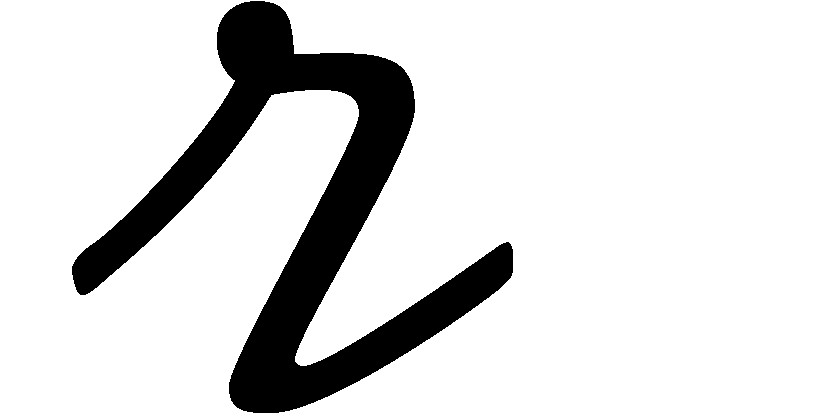
\includegraphics[trim= 1em 0 14em 0,clip]{ScriptR}}$}}}
\def\brcurs{{\mbox{$\resizebox{.09in}{.08in}{
\includegraphics[trim= 1em 0 14em 0,clip]{BoldR}}$}}}

% -----------------------------------------------------------------------

\begin{document}

\raggedright
\footnotesize
\begin{multicols}{3}


% multicol parameters
% These lengths are set only within the two main columns
%\setlength{\columnseprule}{0.25pt}
\setlength{\premulticols}{1pt}
\setlength{\postmulticols}{1pt}
\setlength{\multicolsep}{1pt}
\setlength{\columnsep}{2pt}

\raggedcolumns

\begin{center}
	\Large{\underline{PHYS 350 Formula Sheet}}
\end{center}

\section{Lagrangian Mechanics}
Hamilton's Principle: $\Lagr(\mathbf{q}, \mathbf{\dot{q}}, t)$ minimizes\\
\tab $\Lagr(\mathbf{q}, \dot{\mathbf{q}}, t) \rightarrow S[t] = \int_{t_1}^{t_2} \Lagr(\mathbf{q}, \dot{\mathbf{q}}, t)\,dt$

Euler-Lagrangian Equation:\\
\tab $\ds \dv{t}\left(\pdv{\Lagr}{\dot{q}_i}\right) - \pdv{\Lagr}{q_i} = 0 \qquad i = 1,2,\ldots,s$

Conservation of Energy:\\
\tab $\ds \pdv{\Lagr}{t} = 0$\\
\tab $\ds E = T + U = \sum_{i=1}^{s}\dot{q}_i \pdv{\Lagr}{q_i} - \Lagr$

Conservation of Momentum:\\
\tab $\ds \pdv{\Lagr}{q_i} = 0$\\
\tab $\ds p_i = \pdv{\Lagr}{\dot{q}_i}$

Systems with $s=1$, $\pdv{L}{t} = 0$:\\
\begin{itemize}
\item $\ds \Lagr(q, \dot{q}) = \frac{\alpha(q)\dot{q}^2}{2} - U(q)$
\item $E \geq U(q)$
\item $U(q_o) = E$ are turning points
\item $\ds \int_{0}^{T} dt = \int_{0}^{Q} \frac{1}{\sqrt{\frac{2}{\alpha(q)}(E - U(q))}}dq$
\end{itemize}

\section{Two Body Problem}
Generalized Coordinates:\\
\tab $\brcurs = \vb{r_1} - \vb{r_2}$\\
\tab $\ds \vb{R_\text{CM}} = \frac{m_1\vb{r_1} + m_2 \vb{r_2}}{m_1 + m_2}$\\
\tab $\ds \dot{\vb{r_1}} = \frac{m_2}{m_1 + m_2}\dot{\brcurs} + \vb{R_\text{CM}} \qquad \dot{\vb{r_2}} = -\frac{m_1}{m_1 + m_2}\dot{\brcurs} + \vb{R_\text{CM}}$\\

Lagrangian:\\
\tab $\ds \Lagr = \frac{\mu}{2}\abs{\dot{\brcurs}}^2 + \frac{M}{2}\abs{\dot{\vb{R_\text{CM}}}}^2 - U(\brcurs)$\\
\tab $\ds \mu = \frac{m_1m_2}{m_1 + m_2} \qquad M = m_1 + m_2$

Reduction to independent problems:\\
\tab $\Lagr = \Lagr_\text{CM} + \Lagr_\text{rel}$\\
\tab $\ds \Lagr_\text{CM} = \frac{M}{2}\abs{\dot{\vb{R_\text{CM}}}}^2$\\
\tab $\ds \Lagr_\text{rel} = \frac{\mu}{2}\abs{\dot{\brcurs}}^2 - U(\brcurs)$

Angular Momentum in Polar Coordinates:\\
\tab $\ell = \mu \rcurs^2 \dot{\phi}$

\section{Planetary Motion}
\tab $\ds U(\rcurs) = - \frac{Gm_1m_2}{\rcurs} = -\frac{\alpha}{\rcurs}$

Eccentricity when $\ell \leq 0$:\\
\tab $\ds e = \sqrt{1 + \frac{E_\text{rel}}{U_o}} \qquad U_o = \abs{\min\{U_\text{eff}(\rcurs)\})}$\\
\tab Trajectory = $\begin{cases}
	\text{Constant radius orbit} & e = 0\\
	\text{Ellipse} & 0 < e < 1\\
	\text{Parabola} & e = 1\\
	\text{Hyperbola} & e > 1
\end{cases}$

% Column break
\vfill\null
\section{Small Oscillations}
Equilibrium Point:\\
\tab $\ds \dv{U}{q}\bigg\rvert_{q = q_0} = 0$

Stability Criterion of Equilibrium Point ($s=1$):\\
\tab $\ds \dv[2]{U}{q} > 0$

Stability Criterion of Equilibrium Point ($s \geq 2$):\\
\tab $\ds \pdv{U}{q_i}{q_j} = K_{ij} = K_{ji} \geq 0$

Small Angle Approximation:\\
\tab Taylor expand around equilibrium point of the Lagrangian $q_0$ and keep up to first term that contributes to the Lagrangian.

General Solution to $\ddot{x} = -\omega^2 (x - x_0) + f(t)$:\\
\tab Let $z(t) = \dot{x}(t) + i\omega x(t) \qquad x(t) = x_0 + \Im{z(t)}/\omega$\\
\tab $\ds z(t) = e^{i\omega t}\left[z(0) + \int_{0}^{t} e^{-i\omega \tau} f(\tau)\,d\tau\right]$


\section{Rigid Body Motion}
Kinetic Energy:\\
\tab $T = \frac{M}{2}\abs{\vb{V_0}}^2 + M\vb{\rcurs}_\text{CM} \cdot (\vb{V_0} \cross \vb{\Omega}) + \frac{1}{2}\vb{\Omega}\hat{I_0}\vb{\Omega}$\\
where $\vb{V_o}$ is the velocity of the chosen reference point $\mathcal{O}$, $\vb{\rcurs}_\text{CM} = \vb{R}_\text{CM} - \vb{\rcurs}_\text{O}$ is the position of the CM with respect to $\mathcal{O}$, and $\vb{\Omega}$ is the angular velocity of the body.

Moment of Inertia:\\
\tab $\ds I_{xx}^{(0)} = \int_\mathcal{V} \rho(\vb{r}) (y^2 + z^2)\,dV \qquad I_{xy}^{(0)} = \int_\mathcal{V} \rho(\vb{r}) xy\,dV$

Parallel Axis Theorem:\\
\tab $I_{xx}^{(0)} = I_{xx}^{\text{CM}} + M(d_y^2 + d_z^2)$

% Footer content
\rule{0.3\linewidth}{0.25pt}
\scriptsize\\
Updated \today\\
\href{https://github.com/DonneyF/formula-sheets}{https://github.com/DonneyF/formula-sheets}
\end{multicols}
\end{document}
